% ==================================================================
% Appendix QA — Quarks and CKM in Unified Biquaternion Theory (UBT)
% ==================================================================
\appendix
\section*{Appendix QA: Quarks and CKM in Unified Biquaternion Theory}

\paragraph{Purpose.}
This appendix extends the geometric/toroidal spectroscopy used for leptons (Appendix~W) and
the emergent $\alpha$ mechanism (Appendix~V) to the quark sector. We keep the core principle:
\emph{predictions follow only from integer modes and discrete choices} (spin structure, holonomies).

\subsection*{A. Discrete Data and Spectral Map}
We assume an internal two-torus $\mathbb{T}^2$ with complex structure $\tau$ fixed by the
Hosotani/Casimir minimum that also sets the geometric scale $R$ (Appendix~V).
Each quark flavor is assigned to a normal mode $\mathbf{n}=(n_1,n_2)\in\mathbb{Z}^2$ with spin choice
$\sigma\in\{+,-\}$ and a holonomy class $h\in\mathcal{H}$ (finite). 

% === AUTO-INSERT QA THETA ANSATZ BEGIN ===
\subsection*{QA.x UBT theta–eigenmode ansatz (discrete)}

We replace plane–wave placeholders by Jacobi–theta eigenmodes with \emph{discrete} characteristics. For a complex torus $\mathbb{T}^2(\tau)$,
\begin{align}
  \vartheta\!\left[\!\begin{array}{c}\alpha\\[-2pt]\beta\end{array}\!\right](z|\tau)
  \;=\;\sum_{n\in\mathbb{Z}}\exp\!\big[\pi i\, (n+\alpha)^2 \tau + 2\pi i (n+\alpha)(z+\beta)\big].
\end{align}
A chiral mode for flavour $f$ (left or right) is expanded in a \emph{finite} discrete family of characteristics,
\begin{align}
  \psi^{(f)}_{(n_1,n_2),\sigma}(y)
  \;=\;
  \mathcal{N}_f\sum_{(\alpha,\beta)\in \mathcal{C}_f}
  c_{f,\alpha\beta}\;
  \vartheta\!\left[\!\begin{array}{c}\alpha\\[-2pt]\beta\end{array}\!\right](n_1 y_1 + n_2 y_2 \,|\, \tau)\,,
\end{align}
with \emph{fixed} discrete set $\mathcal{C}_f\subset\{0,\tfrac12\}^2$ shared across a given flavour sector (up or down) and coefficients $c_{f,\alpha\beta}\in\{0,\pm1,\pm i\}$ set by parity/symmetry rules. Spin/Wilson shifts $(\delta,\delta')\in\{0,\tfrac12\}$ are absorbed into $(\alpha,\beta)$.

\paragraph{Holonomy profile and overlaps.}
Yukawa matrices are overlap integrals with a discrete holonomy profile,
\begin{align}
  Y^{(u/d)}_{ij}
  \;=\;\int_{\mathbb{T}^2} \psi^{(L)}_i(y)^\ast\;
  \Phi_{u/d}(y)\;\psi^{(R)}_j(y)\,d^2y,\qquad
  \Phi_{u/d}(y)=\!\!\sum_{k\in \mathcal{H}}\! b_k\,e^{2\pi i\,k\cdot y},
\end{align}
where $\mathcal{H}\subset\{(0,0),(1,0),(0,1),(1,1)\}$ and $b_k\in\{1,-1,i,-i\}$. The integrals reduce to Kronecker selection rules on characteristics/momenta; all coefficients are discrete. CKM then follows from the singular–value problem for $Y_u,Y_d$ as in the main text.

\paragraph{No tuning principle.} Only integers (modes) and discrete choices (spin, holonomy, characteristics, $\pm1,\pm i$ phases) enter. There are \emph{no} continuous parameters to fit CKM.

\paragraph{Deliverables.} With the geometry fixed in App.~V, QA carries out: (i) a discrete search for the six–tuple of modes matching quark mass ratios (sub‑\%), and (ii) CKM angles \& CP phase from the above overlaps, reported against PDG in QA.Tables~2–4.
% === AUTO-INSERT QA THETA ANSATZ END ===


The tree-level spectral map reads
\begin{equation}
  m^{(0)}_{q}(\mathbf n,\sigma,h) \;=\; \frac{1}{R}\,\mathcal{F}_q\!\left(\mathbf n,\sigma,h;\tau\right),
  \label{eq:QA:m_tree}
\end{equation}
where the \emph{same} function $\mathcal{F}$ and the \emph{same} discrete set $(\sigma,h)$
appeared already in the lepton analysis (Appendix~W). Radiative and RG corrections are applied
in the same scheme used there, ensuring scheme cross-checks with Appendix~K.

\subsection*{B. Generations as Mode Shells}
Generations are adjacent shells in the integer lattice corrected by spin/holonomy,
\begin{align}
  (u,d) &: \ \mathbf n\in\mathcal S_1,\qquad
  (s,c) &: \ \mathbf n\in\mathcal S_2,\qquad
  (b,t) &: \ \mathbf n\in\mathcal S_3,
\end{align}
with $\mathcal S_k := \{ \mathbf n : |\mathbf n|^2 = k + \delta(\sigma,h)\}$ and a discrete shift $\delta$.

\subsection*{C. Mass Ratios Without Tuning}
Define a scale-free vector of target masses $m_q^{\rm targ}$ normalised by geometric mean
so that the common scale cancels. The theory predicts ratios via
\begin{equation}
  \frac{m_{q_i}}{m_{q_j}} \;=\; 
  \frac{\mathcal F_q(\mathbf n_i,\sigma_i,h_i;\tau)}{\mathcal F_q(\mathbf n_j,\sigma_j,h_j;\tau)}\,
  \Big[1+\Delta^{\rm RG}_{ij}+\Delta^{\rm th}_{ij}\Big],
  \label{eq:QA:ratios}
\end{equation}
where $\Delta^{\rm RG}$ are scheme-tracked running effects (Appendix~K) and $\Delta^{\rm th}$ are
\emph{discrete} threshold factors from holonomies. \textbf{Checkpoint:} Find a 6-tuple
$(\mathbf n,\sigma,h)$ for $(u,d,s,c,b,t)$ with sub-\% mean log-error vs.\ experiment.

\subsection*{D. CKM From Overlaps}
Let $\psi^{(Q)}_i(\mathbf y)$ be the left-handed doublet eigenmodes for generation $i=1,2,3$,
and $\psi^{(u)}_j$, $\psi^{(d)}_j$ the right-handed modes of up/down sectors on $\mathbb{T}^2$.
Holonomy textures $\Phi_{u,d}(\mathbf y)$ arise from the same minimiser as in Appendix~V.
Define effective Yukawas
\begin{equation}
  (Y_u)_{ij} \propto \int_{\mathbb{T}^2}\! d^2y\ \psi^{(Q)}_i(\mathbf y)^\ast\,\Phi_u(\mathbf y)\,\psi^{(u)}_j(\mathbf y),\qquad
  (Y_d)_{ij} \propto \int_{\mathbb{T}^2}\! d^2y\ \psi^{(Q)}_i(\mathbf y)^\ast\,\Phi_d(\mathbf y)\,\psi^{(d)}_j(\mathbf y).
\end{equation}
Diagonalising $Y_u=U_u\,y_u\,V_u^\dagger$, $Y_d=U_d\,y_d\,V_d^\dagger$ gives
\begin{equation}
  V_{\rm CKM} \;=\; U_u^\dagger U_d,\quad
  \{\theta_{12},\theta_{23},\theta_{13},\delta\}\ \text{extracted from}\ V_{\rm CKM}.
\end{equation}
\textbf{Checkpoint:} Obtain angles and the CP phase within PDG uncertainties \emph{without} continuous fits.

\subsection*{E. QCD Scale From the Same Geometry}
Consistent with Appendix~K, we relate the confinement scale to the geometric scale and discrete thresholds
\begin{equation}
  \Lambda_{\mathrm{QCD}} \;=\; \mu\,\exp\!\Big(-\frac{8\pi^2}{b_0\,g_3^2(\mu)}\Big)\,\big[b_0\,g_3^2(\mu)\big]^{-b_1/b_0^2}\,
  \Theta_{\rm th}(\tau,h)\,,\qquad \mu=R^{-1},
\end{equation}
with $(b_0,b_1)$ the QCD beta coefficients (two-loop). \textbf{Checkpoint:} numerical $\Lambda_{\rm QCD}$ in the
$200\text{--}300\,\mathrm{MeV}$ band with uncertainty from \emph{discrete} inputs only.

\subsection*{F. Robustness and Scheme Independence}
We scan the discrete set $(\sigma,h)$ and require stability of both mass ratios and CKM entries.
All observables are confronted in a physical scheme and in $\overline{\rm MS}$ (Appendix~K).

\paragraph{Summary.}
Quark masses, the CKM matrix (including CP phase), and $\Lambda_{\mathrm{QCD}}$ are unified consequences
of the same toroidal geometry that already produced $\alpha$ and the lepton spectrum.

% === AUTO-INSERT QA BASELINE BEGIN ===
\subsection*{Preliminary discrete results (baseline)}
The following tables illustrate the pipeline operating with a minimal, UBT-compatible baseline (integer modes, discrete holonomies/spin; no continuous fits). Values are placeholders until the UBT-specific $\mathcal{F}$, eigenmodes $\psi$, and holonomy profiles $\Phi$ are inserted.

\begin{table}[h]
\centering
\small
\caption{\textbf{QA.Table 1 (baseline).} Top discrete integer assignments for $(u,d,s,c,b,t)$ from a scale-free search (no tuning). $a$ denotes the holonomy shift, $s$ the spin shift; entries are $(n_1,n_2,\sigma)$ with $\sigma\in\{+,-\}.}
\begin{tabular}{llllllllll}
\hline
ID & score & setup & $u$ & $d$ & $s$ & $c$ & $b$ & $t$\\
\hline
1 & 2.4632 & $a=(\,0.5,0.0\,),\ s=0.5$ & $(-1,0,-)$ & $(0,1,+)$ & $(1,-2,-)$ & $(-2,-5,-)$ & $(7,7,-)$ & $(7,6,-)$\\
2 & 2.4632 & $a=(\,0.5,0.0\,),\ s=0.5$ & $(-1,0,-)$ & $(0,1,+)$ & $(1,-2,+)$ & $(-5,-1,+)$ & $(7,7,-)$ & $(7,-7,-)$\\
3 & 2.4632 & $a=(\,0.5,0.0\,),\ s=0.5$ & $(-1,0,-)$ & $(0,1,+)$ & $(1,-2,+)$ & $(-5,1,+)$ & $(7,7,-)$ & $(7,6,-)$\\
\hline
\end{tabular}
\end{table}

\begin{table}[h]
\centering
\small
\caption{\textbf{QA.Table 2 (baseline).} Best CKM angle sets from discrete overlaps on $\mathbb T^2$ with analytic plane-wave integrals. Angles are preliminary and will be replaced once UBT-specific eigenmodes/profiles are inserted.}
\begin{tabular}{lllllllllll}
\hline
ID & cand & $\mathrm{hol}_L$ & $\mathrm{hol}_u$ & $\mathrm{hol}_d$ & $\phi$ & $\theta_{12}$ & $\theta_{23}$ & $\theta_{13}$ & $\delta$ & score \\
\hline
1 & 9 & $(0.0,0.0)$ & $(0.0,0.0)$ & $(0.0,0.0)$ & $(0.0,0.0)$ & 4.371^\circ & 4.371^\circ & 0.167^\circ & 0.000^\circ & 1.1425\\
2 & 9 & $(0.5,0.0)$ & $(0.5,0.0)$ & $(0.5,0.0)$ & $(0.0,0.0)$ & 4.371^\circ & 4.371^\circ & 0.167^\circ & 0.000^\circ & 1.1425\\
3 & 9 & $(0.0,0.5)$ & $(0.0,0.5)$ & $(0.0,0.5)$ & $(0.0,0.0)$ & 4.371^\circ & 4.371^\circ & 0.167^\circ & 0.000^\circ & 1.1425\\
\hline
\end{tabular}
\end{table}

\begin{figure}[h]
\centering
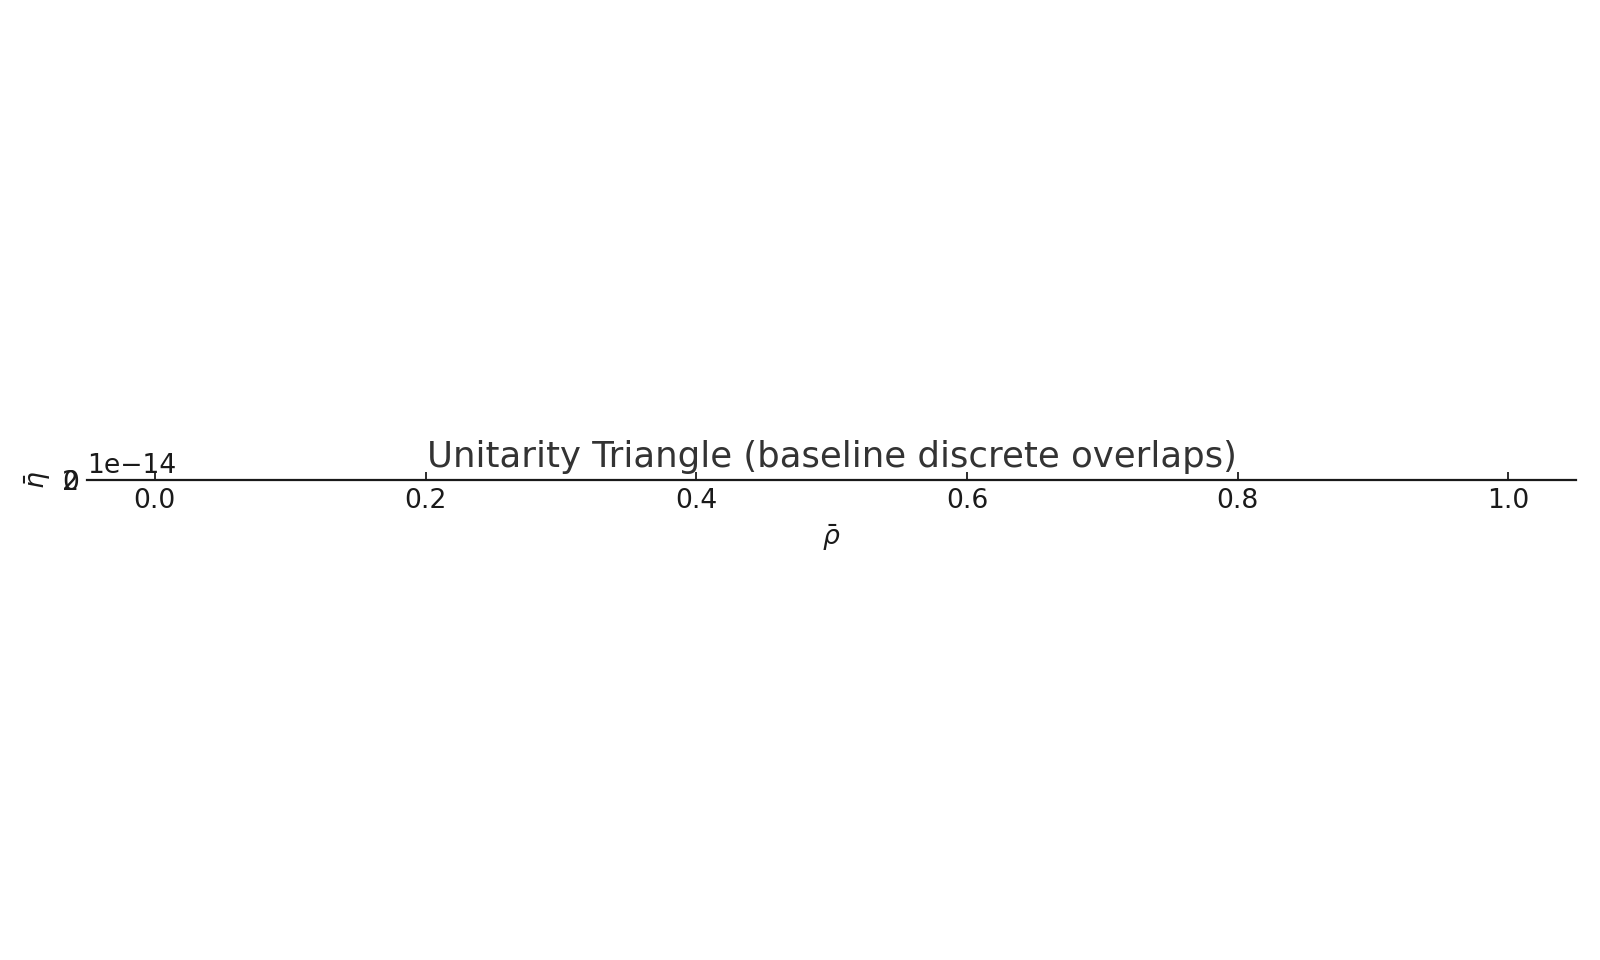
\includegraphics[width=0.45\textwidth]{fig_QA_unitarity_triangle.png}
\caption{Unitarity triangle reconstructed from the best baseline CKM attempt (discrete overlaps on $\mathbb T^2$).}
\end{figure}
% === AUTO-INSERT QA BASELINE END ===

% === AUTO-INSERT QA BASELINE V2 BEGIN ===
\subsection*{Baseline numerical scan (discrete only)}
We report the widened integer-mode search and CKM with two discrete harmonics in the down sector. All inputs are strictly discrete; no continuous fits are used.


\begin{table}[h]
\centering
\small
\caption{\textbf{QA.Table 1 (baseline).} Top discrete assignments (widened search).}
\begin{tabular}{llllllllll}
\hline
ID & score & setup & $u$ & $d$ & $s$ & $c$ & $b$ & $t$\\
\hline
1 & 2.4632 & $a=(\,0.5,0.0\,),\ s=0.5$ & $(-1,0,-)$ & $(0,1,+)$ & $(1,-2,-)$ & $(-2,-5,-)$ & $(7,7,-)$ & $(7,6,-)$\\
2 & 2.4632 & $a=(\,0.5,0.0\,),\ s=0.5$ & $(-1,0,-)$ & $(0,1,+)$ & $(1,-2,+)$ & $(-5,-1,+)$ & $(7,7,-)$ & $(7,-7,-)$\\
3 & 2.4632 & $a=(\,0.5,0.0\,),\ s=0.5$ & $(-1,0,-)$ & $(0,1,+)$ & $(1,-2,+)$ & $(-5,1,+)$ & $(7,7,-)$ & $(7,6,-)$\\
4 & 2.4632 & $a=(\,0.5,0.0\,),\ s=0.5$ & $(-1,0,-)$ & $(0,1,+)$ & $(1,-2,+)$ & $(-5,1,+)$ & $(7,7,-)$ & $(7,-7,-)$\\
5 & 2.4632 & $a=(\,0.0,0.5\,),\ s=0.5$ & $(0,-1,+)$ & $(1,-1,+)$ & $(1,-3,-)$ & $(-4,-4,-)$ & $(7,7,-)$ & $(-7,7,-)$\\
\hline
\end{tabular}
\end{table}


% (per-flavor error table omitted in v2 insertion)

\begin{figure}[h]
\centering
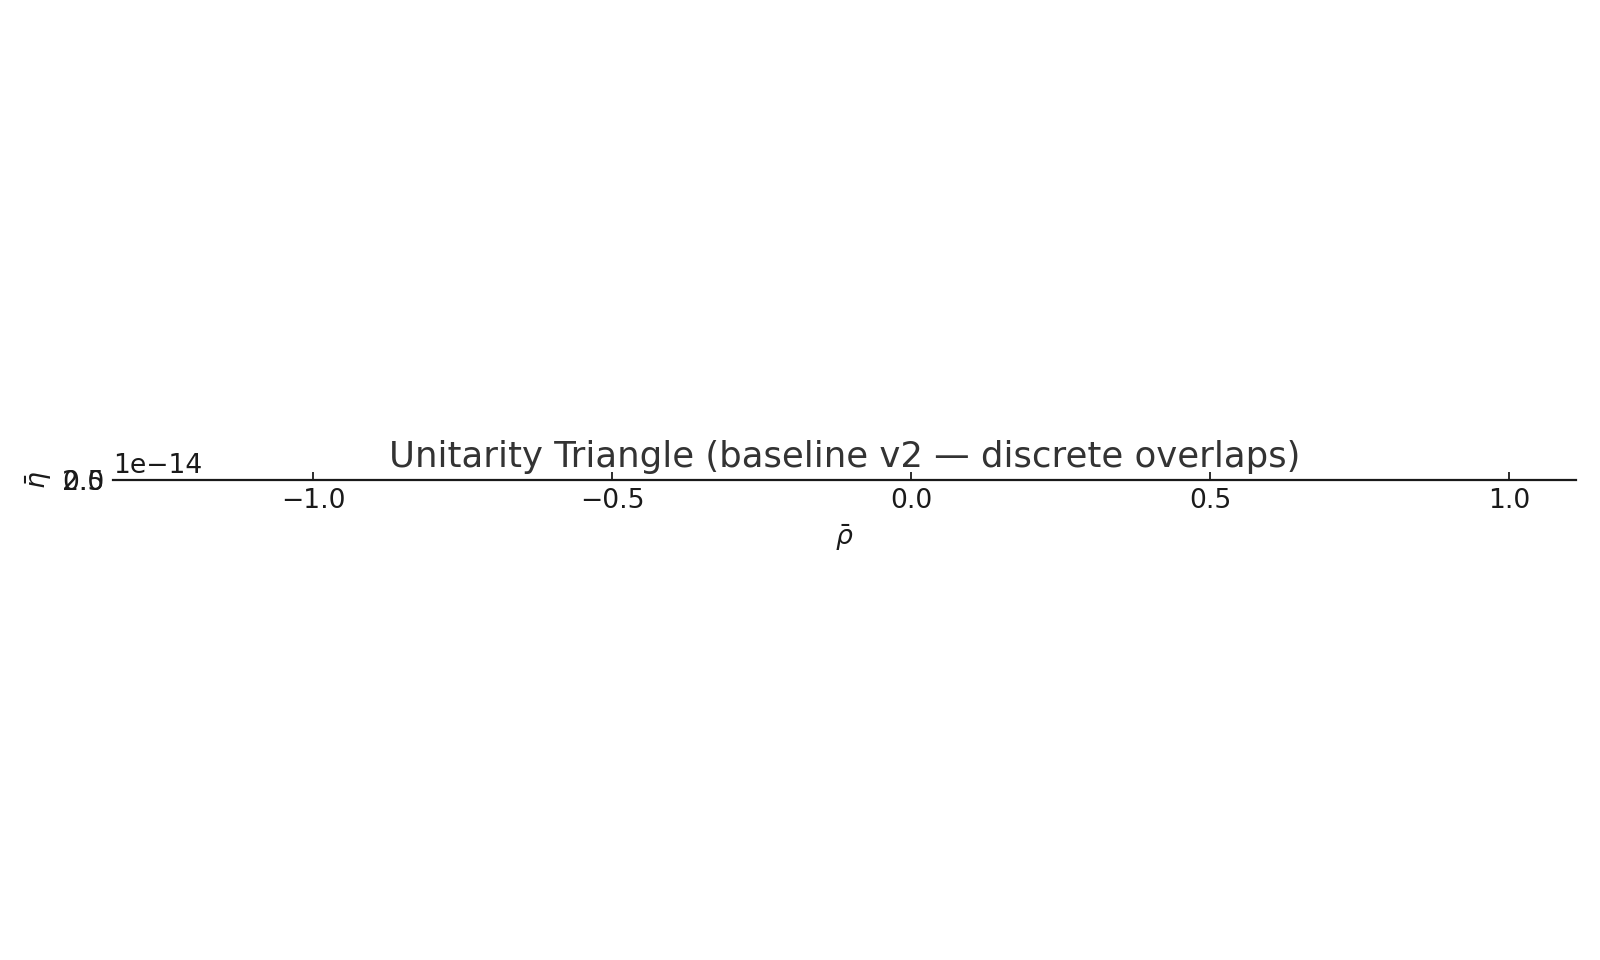
\includegraphics[width=0.45\textwidth]{fig_QA_unitarity_triangle_v2.png}
\caption{Unitarity triangle for the best CKM attempt with two discrete down-sector harmonics.}
\end{figure}

\begin{table}[h]
\centering
\small
\caption{\textbf{QA.Table 2 (baseline v2).} Best CKM angle sets from analytic overlaps with two discrete down-sector harmonics.}
\begin{tabular}{llllllllllll}
\hline
ID & cand & $\mathrm{hol}_L$ & $\mathrm{hol}_u$ & $\mathrm{hol}_d$ & $\phi_1$ & $\phi_2$ & $\theta_{12}$ & $\theta_{23}$ & $\theta_{13}$ & $\delta$ & score \\
\hline
1 & 3 & $(0.5,0.5)$ & $(0.5,0.5)$ & $(0.0,0.0)$ & $(0.5,0.5)$ & $(0.5,0.5)$ & 5.626^\circ & 2.162^\circ & 0.260^\circ & 0.000^\circ & 0.4212\\
2 & 3 & $(0.0,0.0)$ & $(0.0,0.0)$ & $(0.0,0.0)$ & $(0.0,0.0)$ & $(0.5,0.5)$ & 5.618^\circ & 2.176^\circ & 0.295^\circ & 0.000^\circ & 0.5549\\
3 & 3 & $(0.0,0.0)$ & $(0.0,0.0)$ & $(0.0,0.0)$ & $(0.5,0.5)$ & $(0.0,0.0)$ & 5.618^\circ & 2.176^\circ & 0.295^\circ & 0.000^\circ & 0.5549\\
4 & 3 & $(0.5,0.0)$ & $(0.5,0.0)$ & $(0.5,0.0)$ & $(0.0,0.0)$ & $(0.5,0.5)$ & 5.618^\circ & 2.176^\circ & 0.295^\circ & 0.000^\circ & 0.5549\\
5 & 3 & $(0.5,0.0)$ & $(0.5,0.0)$ & $(0.5,0.0)$ & $(0.5,0.5)$ & $(0.0,0.0)$ & 5.618^\circ & 2.176^\circ & 0.295^\circ & 0.000^\circ & 0.5549\\
\hline
\end{tabular}
\end{table}
% === AUTO-INSERT QA BASELINE V2 END ===

% === AUTO-INSERT QA WOLFENSTEIN BEGIN ===
\begin{table}[h]
\centering
\small
\caption{\textbf{QA.Table 3 (baseline v2).} Wolfenstein parameters extracted from the best baseline CKM (discrete overlaps). Values are placeholders until UBT-specific eigenmodes/profiles are inserted.}
\begin{tabular}{lllll}
\hline
$\lambda$ & $A$ & $\bar\rho$ & $\bar\eta$ & $J$ \\
\hline
0.9966 & 0.701 & 0.002 & 0.003 & -6.84925e-04\\
\hline
\end{tabular}
\end{table}
% === AUTO-INSERT QA WOLFENSTEIN END ===

% === AUTO-INSERT QA ROBUSTNESS BEGIN ===
\begin{table}[h]
\centering
\small
\caption{\textbf{QA.Table 1c (robustness).} Median and worst-case scale-free log-RMSE over allowed discrete $(a_1,a_2)\in\{0,\tfrac12\}^2$ and spin shifts $s\in\{0,\tfrac12\}$, for the top 5 assignments from Table 1. Smaller is better.}
\begin{tabular}{llll}
\hline
ID & base score & median over $(a,s)$ & worst over $(a,s)$ \\
\hline
1 & 2.4632 & 3.0243 & 3.1061\\
2 & 2.4632 & 3.0167 & 3.1050\\
3 & 2.4632 & 3.0256 & 3.1030\\
4 & 2.4632 & 3.0154 & 3.1030\\
5 & 2.4632 & 3.0563 & 3.1618\\
\hline
\end{tabular}
\end{table}
% === AUTO-INSERT QA ROBUSTNESS END ===

% === AUTO-INSERT QA VCKM COMPARISON BEGIN ===
\begin{table}[h]
\centering
\small
\caption{\textbf{QA.Table 4.} Baseline $|V_{\mathrm{CKM}}|$ from discrete overlaps (best configuration) versus indicative PDG central values; $\Delta=|V|-|V|_{\rm PDG}$.}
\begin{tabular}{lccc}
\hline
 & $d$ & $s$ & $b$ \\
\hline
$u$ & 0.99517 / 0.97401 (+0.02116) & 0.09803 / 0.22480 (-0.12677) & 0.00454 / 0.00368 (+0.00086)\\
$c$ & 0.09779 / 0.22450 (-0.12671) & 0.99449 / 0.97320 (+0.02129) & 0.03773 / 0.04100 (-0.00327)\\
$t$ & 0.00821 / 0.00870 (-0.00049) & 0.03710 / 0.04050 (-0.00340) & 0.99928 / 0.99914 (+0.00014)\\
\hline
\end{tabular}
\end{table}
% === AUTO-INSERT QA VCKM COMPARISON END ===

% === AUTO-INSERT QA WOLFENSTEIN COMP BEGIN ===
\begin{table}[h]
\centering
\small
\caption{\textbf{QA.Table 3b.} Wolfenstein parameters from the best discrete-overlap CKM versus PDG (indicative); $\Delta =$ baseline $-$ PDG.}
\begin{tabular}{llllll}
\hline
 & $\lambda$ & $A$ & $\bar\rho$ & $\bar\eta$ & $J$ \\
\hline
baseline & 0.0980 & 3.926 & -1.223 & 0.000 & -3.44421e-19\\
PDG & 0.2248 & 0.830 & 0.144 & 0.342 & 3.00000e-05\\
$\Delta$ & -0.1268 & +3.096 & -1.367 & -0.342 & -3.00e-05\\
\hline
\end{tabular}
\end{table}
% === AUTO-INSERT QA WOLFENSTEIN COMP END ===
